%!TEX root = ../../dokumentation.tex

In distributed systems, monitoring can be significantly more difficult than monitoring a monolithic architecture.
Metrics, like latency, traffic, errors and saturation as defined by the \textit{Google Site Reliability Engineering}, are essential from the DevOps perspective, but also for other business units.
In terms of microservices, monitoring makes necessary thresholds visible for scaling and can help to decide whether applications need to be broken down further and scaled individually.
Furthermore showing long term trends, retrospective analysis (e.g. for debugging) and especially alerting are core features of a monitoring system \cite{Ewaschuk.02.12.2019}.

\begin{figure}
	\centering
	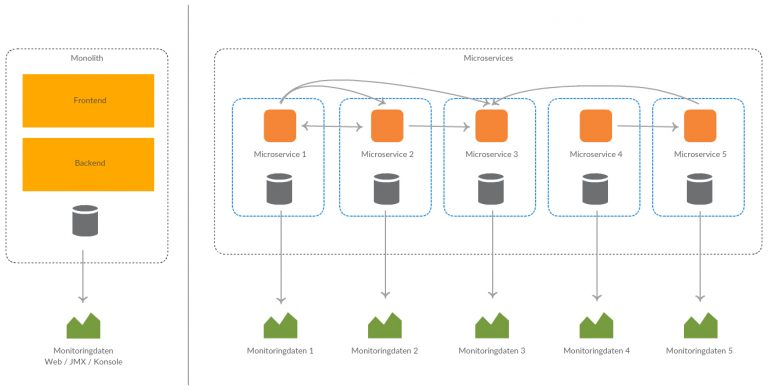
\includegraphics[width=\textwidth, height=0.9\textheight, keepaspectratio]{monitoringMonolithicComparison.jpg}
	\caption{Monolithic monitoring is easier to gather than with microservices~\cite{Fichtner.2016}}
	\label{img:monitoringMonolithicComparison}
\end{figure}

As opposed to a monolith, each microservice generates its own set of monitoring data, these have to be gathered and combined for a meaningful representation.
In order to pinpoint potential issues, metrics and logs from each service (depicted in Figure \ref{img:monitoringMonolithicComparison}) have to be centralized.
This aggregation can be done by either pushing or pulling.
Monitoring frameworks such as \textit{Prometheus} are pulling metrics from services, which have to implement an endpoint and serve data.
The implementation of a metrics endpoint is often called \textit{exporter}.
Time-series databases which do not primarily are built for monitoring (e.g. \textit{InfluxDB}, \textit{Graphite}) have to rely on data collection daemons, which are pushing data to the databases.
Popular daemons for example is the system-metric focused \textit{collectd} or the plugin-driven\textit{Telegraf}, with which a variety of services are supported at once \cite{Fichtner.2016}\cite{Richardson.20.05.2020}\cite{Ewaschuk.02.12.2019}.

In general, aforementioned metric collection daemons are inter-compatible.
Although \textit{Telegraf} would work best with \textit{InfluxDB}\footnote{Referring to the \textit{TICK} stack for centralized alerting and monitoring from the same company \textit{influxdata}: \textit{Telegraf}, \textit{InfluxDB}, \textit{Chronograf} (visualization) and \textit{Kapacitor} (data streaming engine)}, the metric output can be directed to other time-series databases like \textit{Graphite} and even replace the data ingest for \textit{Prometheus} \cite{Loschwitz.2018}.

For this work, the focus is on the time series database itself, as the data aggregation can be interchanged and are mostly compatible to one another.
Furthermore external visualizations such as \textit{Grafana} or \textit{Chronograf} are left out.

\begin{figure}
	\centering
	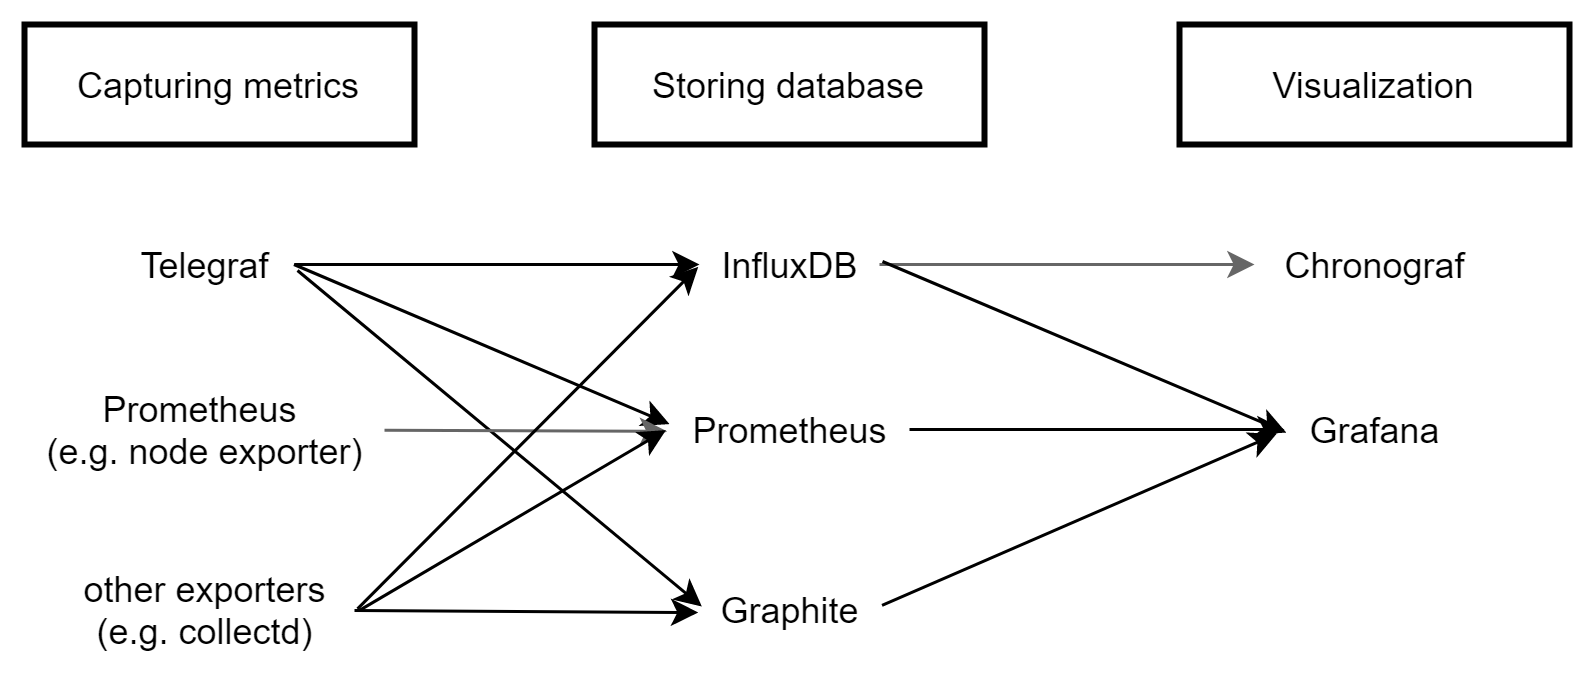
\includegraphics[width=\textwidth, height=0.9\textheight, keepaspectratio]{overviewmonitoring.png}
	\caption{Overview of an selection of popular monitoring technologies}
	\label{img:overviewmonitoring}
\end{figure}

\subsection{Graphite}

As a real-time graphing system based on Python, \textit{Graphite} is able to store numeric time-series data and render graphs.
In order to do so it consists of three main components, as shown in Figure \ref{img:overviewgraphite}, namely the daemon \textit{carbon}, the database library \textit{whisper} and the \textit{graphite webapp} for visualization \cite{Davis.08.05.2020b}.
Unlike \textit{Prometheus} for instance, it relies on inbound metric submissions and does not collect data actively.
Consequently, applications or nodes to be monitored have to be equipped with collection tools, which either communicate over TCP or UDP as plain text, using Python's \textit{pickle} protocol or \ac{AMQP} \cite[p.~49]{Dixon.2017}\cite{Davis.08.05.2020c}.

In most cases, however, tools already support the format, as seen in Listing \ref{listing:graphitemessage}, and handle metrics export and communication with \textit{Graphite}'s \textit{carbon-cache}.
An extensive list of currently supported collectors as well as further compatible tools, which should be used in conjunction, can be found in the \textit{Graphite} documentation \cite{Davis.08.05.2020d}.

\begin{lstlisting}[caption=Graphite Message Format, label=listing:graphitemessage]
metric_path value timestamp
\end{lstlisting}

\begin{lstlisting}[caption=Graphite's dot oriented naming scheme, label=listing:graphitemetricnaming]
api_server_http_requests_total.post.500.tracks.sample1 
\end{lstlisting}

The logical component \textit{carbon} as shown in Figure \ref{img:overviewgraphite} consists of a relay, an aggregator and the actual required \textit{carbon-cache}.
The latter represents the core to accept metrics over aforementioned protocols.
A \textit{Graphite} message (if not bundled using Python's \textit{pickle}) contains the metric namespace to be populated (\textit{metric\_path}), the \textit{value} and a timestamp, as seen in Listing \ref{listing:graphitemessage} \cite{Davis.08.05.2020c}.
\textit{Graphite}'s metrics naming is dot oriented and implies hierarchy.
In Listing \ref{listing:graphitemetricnaming} an exemplary metric name is given for HTTP POST requests with the \textit{response code 500} landing on the \textit{/tracks} endpoint.

\begin{figure}
	\centering
	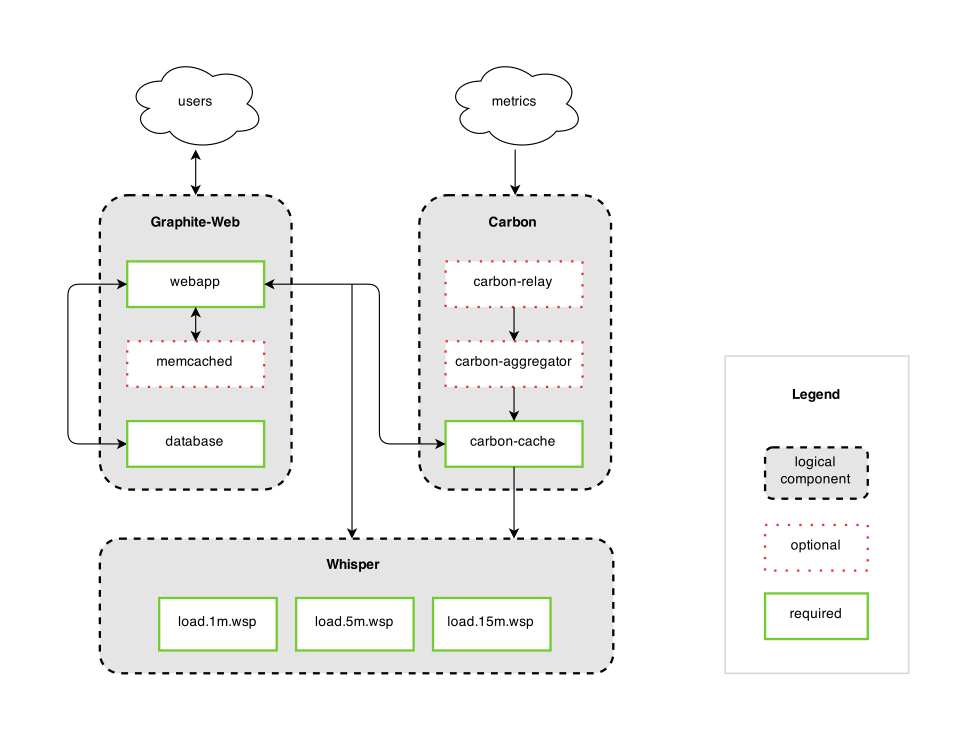
\includegraphics[width=\textwidth, height=0.8\textheight, keepaspectratio]{graphiteoverview.png}
	\caption{Overview of Graphite's architecture \cite{Davis.08.05.2020}}
	\label{img:overviewgraphite}
\end{figure}

The relay is needed for scaling the \textit{carbon-cache} processes, which can be on different servers.
However, in practice typical load balancers such as \textit{HAProxy} are used in front of the logical component \textit{carbon} as a whole to split metrics and thus scaling \textit{Graphite} \cite{Dubiel.29.05.2020}.
In order to reduce load, an aggregator can be used to buffer metrics before saving them using \textit{whisper}, which is a fixed sized database file format for datapoints \cite[p.~52]{Dixon.2017}.
Each \textit{*.wsp} file in\textit{whisper} needs corresponding scheme definitions for retention policies and precision settings.
These settings can be used to duplicate metrics with a lower precision to save space, while removing the original after its retention duration \cite[p.~55]{Dixon.2017}.
Lastly \textit{graphite-web} can be used to visualize data in real-time from the \textit{whisper} storage and \textit{carbon-cache} simultaneously.


The performance of \textit{Graphite} is generally bound to the \ac{I/O} performance of the system.
Usually this is mitigated by increasing the disk array, placing aggregators and load balance between them.
Although this way of vertical scaling is supported well, horizontal scaling can be cumbersome, as one has to decide between redundancy (replication factor) or high performance by utilizing consistent hashing across all instances \cite[p.~57ff.]{Dixon.2017}.
Possible currently used and common alternatives to avoid the scaling problem, are replacing the underlying \textit{whisper} storage engine (e.g. with \textit{InfluxDB}) or replacing the relay with alternative implementations (e.g. \textit{carbon-relay-ng} written in Go) to achieve higher performance.

\subsection{InfluxDB}

\textit{InfluxDB} is a time series database and provides an SQL-like query language (\textit{InfluxQL}) for data interaction, unlike \textit{Graphite}.
The company \textit{influxdata}, provides an open-source version (\textit{InfluxDB OSS}) and a commercial version (\textit{InfluxDB Enterprise}).
Although \textit{InfluxDB} has a higher performance than \textit{Graphite}, as shown in an extensive technical paper, including benchmarks, and thus would be a very good database for monitoring usages, it can not be taken into consideration due to missing features \cite{influxdata.2019}.
The main reason is the missing clustering option for the database.
In the open-source variant, high availability is not guaranteed and horizontal scalability through sharding is not available.
Especially when deploying a high demanding application, such as a large management application, operating \textit{InfluxDB} on a single node seems to be insufficient \cite{influxdata.2020}.
Consequently, no overview will be given here as non open-source and especially paid features are not in the scope of research, leaving \textit{InfluxDB OSS} not suitable.

\subsection{Prometheus}

Similar to \textit{Graphite}, \textit{Prometheus} is primarily used for system monitoring and includes a time-series database and a monitoring system.
Currently \textit{Prometheus} is part of the \textit{Cloud Native Computing Foundation} and open source.
Besides storing and retrieving metrics, it also includes an alerting system and a web \ac{UI}.
Moreover, \textit{Prometheus} has a broad support of clients, by using exporters on the client side.
Unlike other monitoring solutions which depend on passive listeners and clients pushing metrics to the service, \textit{Prometheus} mainly relies on pulling \cite{Berman.2018}\cite{PrometheusAuthors.30.05.2020}.

\begin{figure}
	\centering
	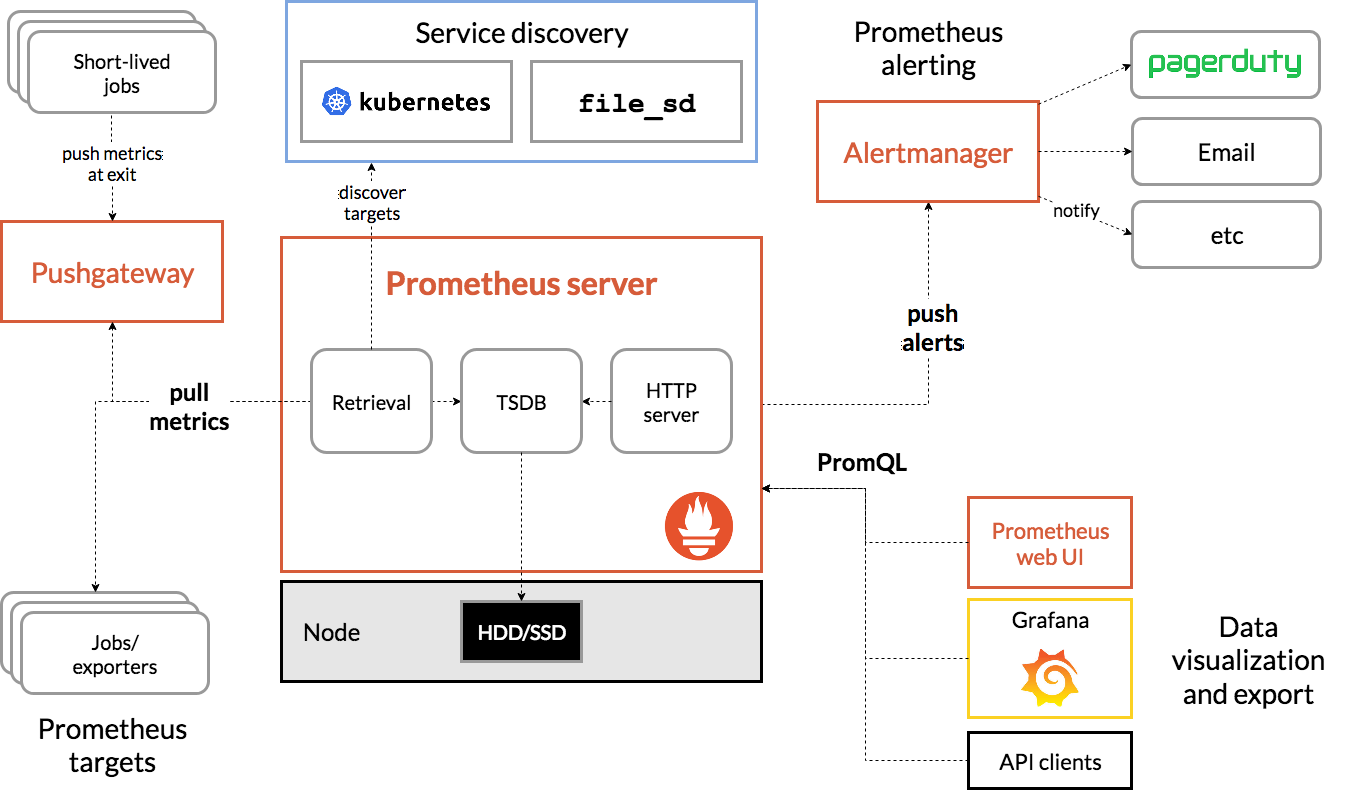
\includegraphics[width=\textwidth, height=0.8\textheight, keepaspectratio]{prometheusoverview.png}
	\caption{Overview of Prometheus' architecture \cite{PrometheusAuthors.30.05.2020}}
	\label{img:prometheusoverview}
\end{figure}

As seen in Figure \ref{img:prometheusoverview} metrics are pulled from \textit{Prometheus} target, which expose their metric on a \ac{HTTP} endpoint.
Consequently, \textit{Prometheus} handles data scraping itself and stores it in an internal \ac{TSDB}.
Although the concept of pulling is favored, \textit{Prometheus} is compatible with existing \enquote{pushing} clients as well, by utilizing the intermediary \textit{Pushgateway}, which stores and aggregates data.
For the active pulling, the endpoints can either be static, or be discovered by utilizing external service registries.
Apart from collecting and storing metrics, events and alerts can be configured in the \textit{Alertmanager} for sending notifications.
Lastly, external visualizations and clients can communicate with \textit{Prometheus} using its own \textit{Prometheus Query Language (PromQL)} \cite{PrometheusAuthors.30.05.2020}.

Similarly to \textit{Graphite}'s \textit{whisper}, time series are stored locally and are grouped into blocks.
With \textit{Prometheus}, incoming samples are kept in memory first and are secured with a write-ahead-log, before being persisted and grouped into two hour blocks.
Like \textit{Graphite}, retention policies and compression options are available for the \ac{TSDB} format.
This approach however, can limit the scalability and durability of the system, as the local storage is bound to the performance of a single node, especially with the concept of node autonomy found in \textit{Prometheus}.
Possible solutions are to replace the \ac{TSDB}, against remote storage systems, to which \textit{Prometheus} communicates with protocol buffers over \ac{HTTP} \cite{PrometheusAuthors.30.05.2020b}.

\textit{Prometheus} is generally known for the variety of exporters available for \acp{API}, messaging systems, hardware related metric systems and also databases. (see \cite{PrometheusAuthors.30.05.2020c} for an extensive list)
Instead of converting existing metrics to the \textit{Prometheus} exposition format, using aforementioned exporters, client libraries are available as well, with which metrics of an application are defined and exposed.

Similar to the \textit{Graphite} message format (see Listing \ref{listing:graphitemessage}), one can also write raw messages, which include the metric name, value and timestamp \cite{PrometheusAuthors.30.05.2020d}.
However, the data model of \textit{Prometheus} allows more complex metadata models by including \enquote{labels}, i.e. key values pairs.
Depicted in Listing \ref{listing:prometheusmessage} is an exemplary metric of the number of HTTP POST requests with the \textit{response code 500} to the \textit{/tracks} endpoint.
This explicit multidimensionality allows greater flexibility compared to the implicit dimension encoding found in \textit{Graphite}, which makes progressive changes in naming difficult to maintain (compare Listings \ref{listing:graphitemetricnaming} and \ref{listing:prometheusmessage}) \cite{Berman.2018}\cite{PrometheusAuthors.30.05.2020e}.

\begin{lstlisting}[caption=Prometheus exposition format with example, label=listing:prometheusmessage]
// syntax: metric_name{label_name = label_value, ...} value [timestamp]

api_server_http_requests_total{method="POST",handler="/tracks",status="500"} 34
\end{lstlisting}

With the aforementioned concept of write ahead logs for instance, reliability is one of the core principles.
The autonomy of each \textit{Prometheus} instance allows access to metrics, even under failure conditions.
However, just like \textit{Graphite}, scaling may be difficult.
A common approach is splitting up the metrics to be monitored and the \textit{Prometheus} instance bound to it, which would value the autonomy aspect.
Alternatively \textit{Prometheus} can scale horizontally by sharding , which means that a subset of metrics are scraped by slaves (partitioning) and are then federated by the master \cite{Brazil.2015}\cite{Berman.2018}.
